\section{التحكم عالي المستوى \LR{High-Level Control (HLC)}}
\label{sec:high_level_control}

يمثل التحكم عالي المستوى \LR{High-Level Control (HLC)} الطبقة التي تتعامل مع هدف الحركة في الفضاء الكارتزي، أي مع موضع النهاية المنفذة بدلاً من التعامل المباشر مع إشارات الجهد أو العزم للمشغلات. وبما أن خوارزميات التحكم منخفض المستوى \LR{LLC} قد دُرست سابقاً من ناحية تتبع مراجع المفاصل، فإن هذا القسم يركز على توليد هذه المراجع انطلاقاً من موضع النهاية المنفذة المطلوب.

تعتمد الفكرة العامة على إعطاء الموضع المطلوب:

\[
X_{ref} =
\begin{bmatrix}
x_{ref} \\
y_{ref} \\
z_{ref}
\end{bmatrix}
\]

ثم استخدام الحل الحركي العكسي \LR{Inverse Kinematics (IK)} لحساب زوايا المفاصل المرجعية \(q_{ref}\). بعد ذلك تُمرر هذه الزوايا إلى طبقة \LR{LLC} من أجل تنفيذ الحركة على مستوى المفاصل، بينما يُستخدم الحل الحركي الأمامي \LR{Forward Kinematics (FK)} للتحقق من الموضع الناتج للنهاية المنفذة.

\subsection{المخطط العام للتحكم عالي المستوى}
\label{subsec:general_hlc_diagram}

يوضح الشكل \ref{fig:general_hlc_block_diagram} المخطط العام لطبقة التحكم عالي المستوى. تتم مقارنة الموضع المطلوب \(X_{ref}\) مع الموضع الناتج \(X\)، ثم يُستخدم الخطأ الكارتزي \(E_X\)    لتوليد الموضع المطلوب للحل الحركي العكسي. بعد ذلك يقوم بلوك \LR{IK} بتحويل هذا الموضع إلى مراجع مفصلية \(q_{ref}\)، والتي تنتقل إلى طبقة \LR{LLC} ثم إلى نموذج الذراع.

\begin{figure}[H]
\centering
\resizebox{\textwidth}{!}{
\begin{tikzpicture}[
    block/.style={
        draw,
        rectangle,
        minimum width=2.6cm,
        minimum height=1.15cm,
        align=center
    },
    sum/.style={
        draw,
        circle,
        minimum size=0.65cm,
        inner sep=0pt
    },
    arrow/.style={
        -{Latex[length=2mm]},
        thick
    },
    node distance=1.0cm
]

% =========================================================
% Main path nodes
% =========================================================

\node[block] (xref) {
\begin{tabular}{c}
\(X_{ref}\)\\
\LR{Desired Position}
\end{tabular}
};

\node[sum, right=1.0cm of xref] (sum1) {\(\Sigma\)};

\node[block, right=1.0cm of sum1] (controller) {
\begin{tabular}{c}

\LR{Controller}
\end{tabular}
};

\node[block, right=1.0cm of controller] (ik) {
\begin{tabular}{c}
\LR{IK}\\
\LR{Inverse Kinematics}
\end{tabular}
};

\node[block, right=1.0cm of ik] (llc) {
\begin{tabular}{c}
\LR{LLC}\\
\LR{Low-Level Control}
\end{tabular}
};

\node[block, right=1.0cm of llc] (robot) {
\begin{tabular}{c}
\LR{Robot Plant}\\
\LR{Dynamic Model}
\end{tabular}
};

% =========================================================
% Feedback path nodes
% =========================================================

\node[block, below=1.55cm of robot] (fk) {
\begin{tabular}{c}
\LR{FK}\\
\LR{Forward Kinematics}
\end{tabular}
};

\path (sum1 |- fk) node[block] (sensor) {
\begin{tabular}{c}
\LR{Sensors}
\end{tabular}
};

% =========================================================
% Main path arrows
% =========================================================

\draw[arrow] (xref) -- (sum1);
\draw[arrow] (sum1) -- node[above] {\(E_X\)} (controller);
\draw[arrow] (controller) -- node[above] {\(X_{cmd}\)} (ik);
\draw[arrow] (ik) -- node[above] {\(q_{ref}\)} (llc);
\draw[arrow] (llc) -- node[above] {\(q_i\)} (robot);

% =========================================================
% Feedback path arrows
% =========================================================

\draw[arrow] (robot.south) -- (fk.north);
\draw[arrow] (fk.west) -- node[below] {\(X\)} (sensor.east);
\draw[arrow] (sensor.north) -- (sum1.south);

% =========================================================
% Sum signs
% =========================================================

\node[above left=-0.05cm and -0.05cm of sum1] {\(+\)};
\node[below left=-0.05cm and -0.05cm of sum1] {\(-\)};

\end{tikzpicture}
}
\caption{\centering{المخطط العام لطبقة التحكم عالي المستوى \LR{HLC}}}
\label{fig:general_hlc_block_diagram}
\end{figure}

يمكن تلخيص تسلسل العمل في طبقة التحكم عالي المستوى كما يلي:

\[
X_{ref}
\rightarrow
\text{\LR{HLC}}
\rightarrow
\text{\LR{IK}}
\rightarrow
q_{ref}
\rightarrow
\text{\LR{LLC}}
\rightarrow
q
\rightarrow
\text{\LR{FK}}
\rightarrow
X
\]

اعتمد هذا الجزء على النموذج الحركي المبني سابقاً باستخدام معاملات \LR{DH}، حيث استُخدم هذا النموذج لحساب الحل الحركي العكسي وتوليد مراجع المفاصل. بعد ذلك تُمرر هذه المراجع إلى طبقة \LR{LLC}، والتي تمثل مرحلة تنفيذ الحركة على مستوى المفاصل قبل انتقالها إلى نموذج الذراع \LR{Robot Plant}. وفي نهاية السلسلة، يتم استخدام الحل الحركي الأمامي \LR{FK} لحساب الموضع الناتج للنهاية المنفذة والتحقق من مطابقته للموضع المطلوب.






\subsection{بناء نموذج التحكم عالي المستوى في بيئة \LR{MATLAB/Simulink}}
\label{subsec:hlc_simulink_model}

بعد توضيح البنية العامة لطبقة التحكم عالي المستوى، تم بناء النموذج العملي في بيئة \LR{MATLAB/Simulink}. يعتمد النموذج على إدخال الموضع المطلوب للنهاية المنفذة في الفضاء الكارتزي بوحدة السنتيمتر:

\[
X_{ref} =
\begin{bmatrix}
x_{ref} \\
y_{ref} \\
z_{ref}
\end{bmatrix}
\]

ثم يتم تمرير هذه القيم إلى بلوك الحل الحركي العكسي \LR{IK}. تم بناء نموذج \LR{IK} اعتماداً على معاملات \LR{DH} الخاصة بالذراع، وباستخدام مكتبة \LR{Robotics System Toolbox} في \LR{MATLAB} لحساب زوايا المفاصل الموافقة للموضع المطلوب.

يعطي بلوك \LR{IK} خمس زوايا مرجعية للمفاصل:

\[
q_{ref} =
\begin{bmatrix}
q_{1,ref} \\
q_{2,ref} \\
q_{3,ref} \\
q_{4,ref} \\
q_{5,ref}
\end{bmatrix}
\]

وتكون هذه الزوايا بوحدة الراديان \LR{rad}. بعد ذلك تنتقل هذه المراجع إلى طبقة \LR{LLC}، والتي تقوم بتهيئة وتنفيذ الحركة على مستوى المفاصل قبل تمريرها إلى نموذج الذراع.

تم استخدام نموذج الذراع المبني في \LR{Simscape Multibody} من أجل تنفيذ الحركة والتحقق من سلوك الذراع في بيئة محاكاة فيزيائية. كما تم إضافة بلوك للحل الحركي الأمامي \LR{FK} بعد نموذج الذراع، وذلك من أجل حساب الموضع الناتج للنهاية المنفذة ومقارنته مع الموضع المطلوب.

يوضح الشكل \ref{fig:hlc_simulink_model} نموذج التحكم عالي المستوى كما تم بناؤه في بيئة \LR{Simulink}.

\begin{figure}[H]
    \centering
    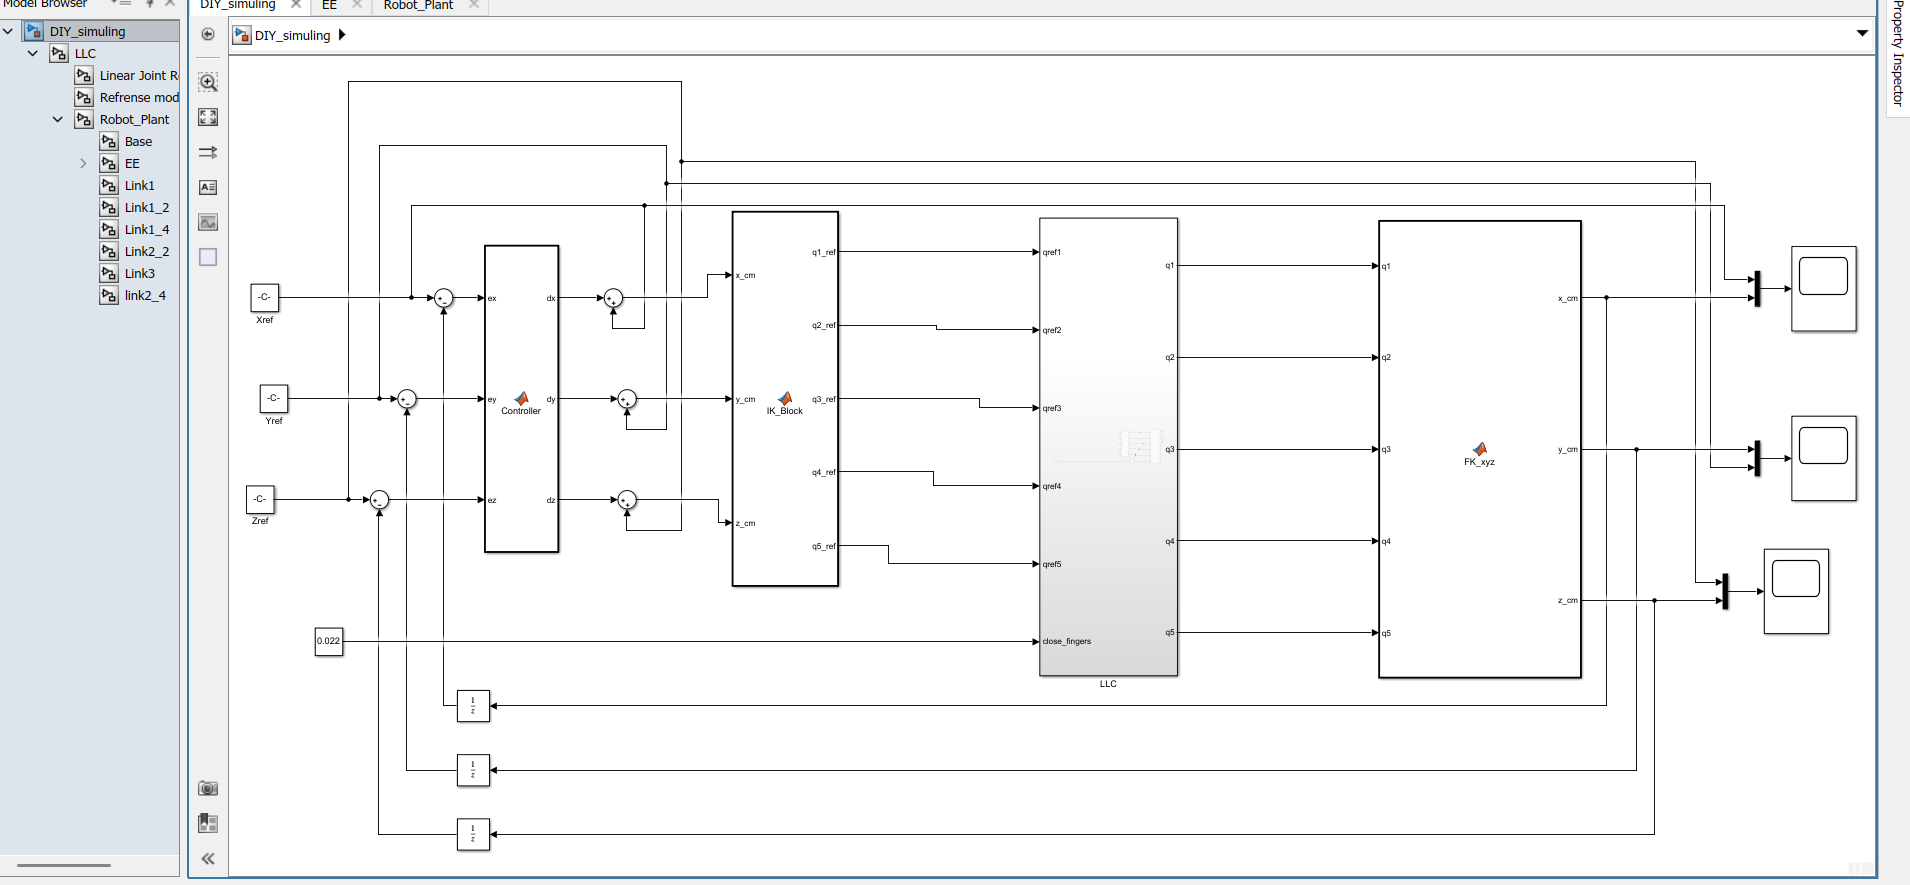
\includegraphics[width=\textwidth]{resources/images/HLC_simulink_model}
    \caption{\centering{نموذج التحكم عالي المستوى في بيئة \LR{Simulink}}}
    \label{fig:hlc_simulink_model}
\end{figure}







\subsection{نتائج تتبع موضع النهاية المنفذة}
\label{subsec:hlc_results}

بعد بناء نموذج التحكم عالي المستوى في بيئة \LR{Simulink}، تم اختبار قدرة النموذج على تحويل الموضع المطلوب للنهاية المنفذة إلى مراجع مفصلية مناسبة، ثم تنفيذ هذه المراجع عبر نموذج الذراع. تم في هذه التجربة إدخال موضع مرجعي ثابت للنهاية المنفذة في الفضاء الكارتزي، ثم حساب زوايا المفاصل المقابلة باستخدام بلوك الحل الحركي العكسي \LR{IK}.

يوضح الشكل \ref{fig:hlc_response} استجابة موضع النهاية المنفذة في المحاور الثلاثة \(x\)، \(y\)، و \(z\). تم حساب الموضع الناتج باستخدام الحل الحركي الأمامي \LR{FK} اعتماداً على زوايا المفاصل الخارجة من نموذج الذراع، ثم تمت مقارنته مع الموضع المرجعي المطلوب.

\begin{figure}[H]
    \centering
    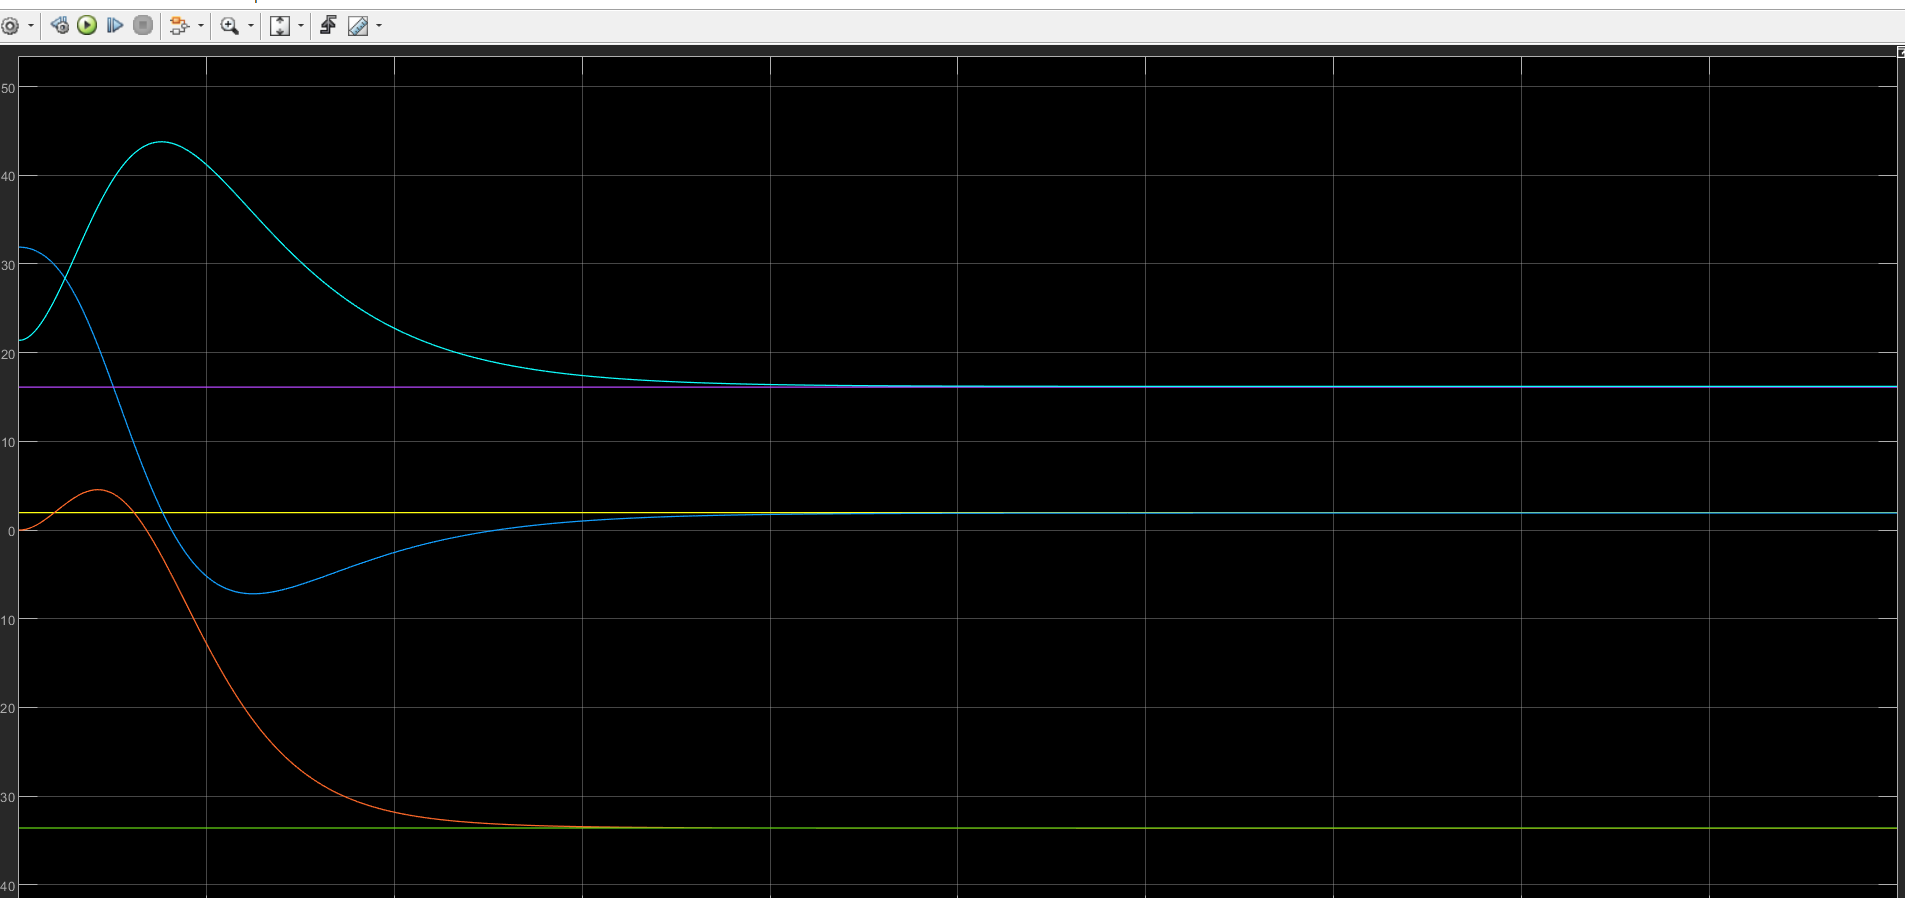
\includegraphics[width=\textwidth]{resources/images/HLC_response}
    \caption{\centering{استجابة موضع النهاية المنفذة باستخدام طبقة التحكم عالي المستوى \LR{HLC}}}
    \label{fig:hlc_response}
\end{figure}

من الشكل يمكن ملاحظة أن الموضع الناتج للنهاية المنفذة يتقارب مع القيم المرجعية المطلوبة بعد مرحلة انتقالية أولية. تعود هذه المرحلة الانتقالية إلى تأثير نموذج توليد المراجع الحركية للمفاصل وإلى انتقال الذراع من الوضع الابتدائي إلى الوضع المطلوب. وبعد انتهاء هذه المرحلة، تستقر الإحداثيات الكارتزية حول القيم المطلوبة، مما يدل على أن طبقة \LR{HLC} استطاعت توليد مراجع مفصلية مناسبة اعتماداً على الموضع المطلوب للنهاية المنفذة.

تؤكد هذه النتيجة أن سلسلة التحكم المستخدمة:

\[
X_{ref}
\rightarrow
\text{\LR{IK}}
\rightarrow
q_{ref}
\rightarrow
\text{\LR{LLC}}
\rightarrow
q
\rightarrow
\text{\LR{FK}}
\rightarrow
X
\]

قادرة على ربط الموضع الكارتزي المطلوب بحركة المفاصل، والتحقق من وصول النهاية المنفذة إلى الموضع المطلوب داخل نموذج المحاكاة.
\\
تم ارفاق بعض الفيديوهات يوضح عملية انتقال الذراع للنقطة المطلوبة :
 \\


\begin{center}
\href{file:///D:/Projects/latex/Studying_DIY_Arm/resources/images/HLC_response_P1.mp4}
{ هنا}
\end{center}

\begin{center}
\href{file:///D:/Projects/latex/Studying_DIY_Arm/resources/images/HLC_response_P2.mp4}
{ هنا}
\end{center}

\begin{center}
\href{file:///D:/Projects/latex/Studying_DIY_Arm/resources/images/HLC_response_P3.mp4}
{ هنا}
\end{center}